\documentclass[12pt]{article}
\usepackage{ctex}%引入中文字符的包
\usepackage{enumerate}%引用标号需要引入的包
\usepackage{amsmath}
%\usepackage{array}
\usepackage{graphicx}%用来在文档中插入图片
\usepackage{caption}%修改图注相关
\usepackage{subfigure}%用来插入并列的图片
\usepackage{float}%确定图片是否为浮动,而不是在一个固定的地方
\usepackage[a4paper,left=31.8mm,right=31.8mm,top=25.4mm,bottom=25.4mm]{geometry}
\begin{document} 
\begin{titlepage}
\begin{center}      
{\Huge \bfseries 机器学习实验报告}\\[1cm]
{\Large \bfseries 主成分分析(Principal Component Analysis)}\\[10cm]
{\Large 姓名:秦海滨}\\[1cm]
{\Large 学号:1180300523}\\[8cm]
{\Large 2020年11月10号}
\end{center}
\end{titlepage}
\newpage
\tableofcontents
\newpage
\section{实验目的}
实现一个 PCA 模型,能够对给定数据进行降维(即找到其中的主成分)。\par
\section{实验要求及环境}
\subsection{实验要求}
\begin{enumerate}
    \item 人工生成一些数据(如三维数据),让它们主要分布在低维空间中。如首先让某个维度的方差远小于其它维度,然后对这些数据旋转。生成这些数据后,用你的 PCA 方法进行主成分提取。\par
    \item 找一个人脸数据(小点样本量),用你实现 PCA 方法对该数据降维,找出数据主成分,然后用这些主成分对每一副人脸图像进行重建,比较一些它们与原图像有多大差别(用信噪比衡量)。\par
\end{enumerate}
\subsection{实验环境}
\noindent 操作系统:Windows10 \par
\noindent 开发环境:Spider 4.1.4,Python 3.8 \par
\section{基本思想}
PCA(Principal Component Analysis)是一种常见的数据分析方式,一般用于高维数据的降维,可用于提取数据的主要特征分量。其数学推导一般从最大可分性和最近重构性进行,前者的优化条件表示需要在降维后数据间的方差最大,后者的优化条件表示划分出的点与划分平面(投影面)的距离最小。\par
我们可以认为PCA完成了将高维的数据点投影到低维的超平面上,其投影结果既要满足样本点在这个超平面上的投影尽可能的分开(方差较大),也要满足样本点到这个超平面的距离足够近。\par
首先,我们对于需要进行PCA的数据进行中心化,即保证其均值为0,公式如下:\par
\[x_i=x_i-\frac{1}{m}\sum_{j=1}^mx_j\]\par
即对每一个样本点减去其样本均值,这样能保证对经过中心化后的数据常规的线性变换即是绕着原点的旋转变化。而且这样能够保证以一种较为简明的形式表示样本的协方差矩阵,如下:
\[\varSigma=E[(X-E[X])(X-E[X])^T]=\frac{1}{m}XX^T\]\par
设使用的投影坐标系的标准正交向量基为$W=\{w_1,w_2,\dots,w_d\},d<n$,这样每个样本点$x_i$降维后得到的坐标为$z_i=\{z_i1;z_i2;\dots;z_id\}$。其中,$z_{ij}=w_j^Tx_i$,表示$x_i$在d维坐标系下第j维的坐标。若基于$z_i$来重构$x_i$,我们会得到$\hat{x}=Wz$。则考虑整个训练集上,原样本点$x_i$与基于投影重构的样本点$\hat{x}_i$之间的距离为:
\[\sum_{i=1}^m||\sum_{j=1}^dz_{ij}w_j-x_i||_2^2\]\par
根据最近重构性,该式应被最小化。考虑到$w_j$是标准正交基,$\sum_{i}x_ix_i^T$是协方差矩阵,我们可以得到上述距离公式与$W^TXX^TW$的迹成反比,这就是我们需要优化的目标。我们要使可重构性最小,则要使矩阵$W^TXX^TW$的迹最大。\par
同样的,从最大可分性出发。样本点$x_i$在降维平面上的投影是$W_Tx_i$,样本点的协方差矩阵为$\sum_iW^Tx_ix_i^TW$,这与最近重构性得出的优化目标相同!\par
我们对于优化目标式采用拉格朗日乘子法,有:
\[XX^Tw_i=\lambda_iw_i\]\par
于是,我们只需要对协方差矩阵$XX^T$进行特征值分解,将所求的的特征值排序:$\lambda_1\geq\lambda_2\geq\dots\geq\lambda_n$,从中取出前d个特征值对应的特征向量构成$W^*=(w_1,w_2,...,w_d)$,这就是主成分分析的解。\par
\section{数据的生成}
\subsection{三维数据的生成}
为了能够明显地可视化,我们选择了三维数据进行数据分析。能够在给定了数据在三个特征维度上的均值和协方差矩阵,利用库中的生成函数生成出需要降维的数据。
\subsection{人脸数据读取}
我从一些热门电影的演员中截取的人脸图片,将其裁剪为正方形便于后续计算。
\section{实验结果分析}
\subsection{三维数据降维后的结果}
三维数据降维到二维之后会投影到一个平面上,程序运行结果如下:\par
\begin{figure}[H]
    \centering
    \subfigure[三维数据降维到二维的结果(平面正视图)]{
        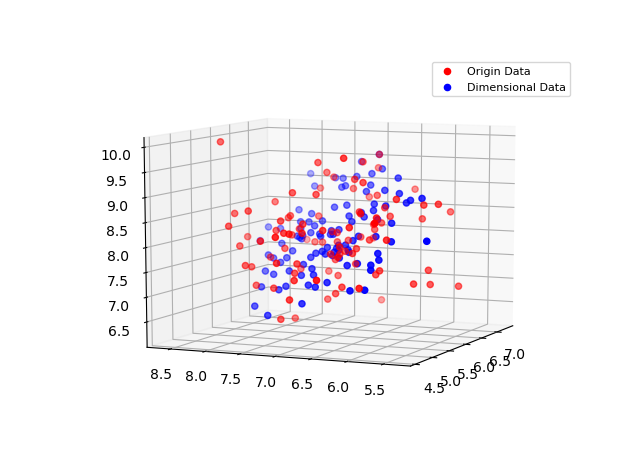
\includegraphics[width=0.7\textwidth]{3d-2d-1.png}
    }
\end{figure}
\begin{figure}[H]
    \centering
    \subfigure[三维数据降维到二维的结果(平面侧视图)]{
        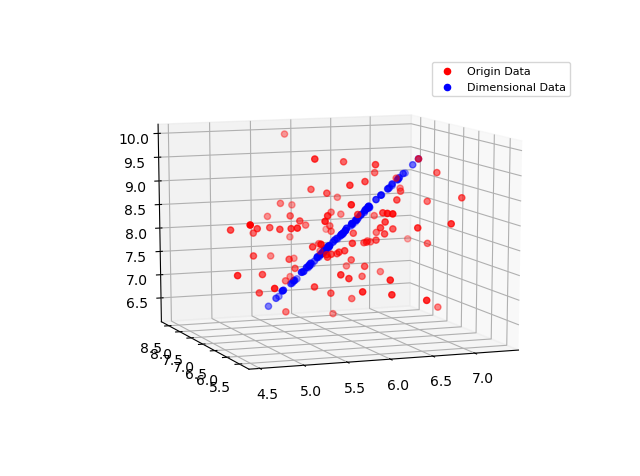
\includegraphics[width=0.7\textwidth]{3d-2d-2.png}
    }
\end{figure}
我们也可以尝试将数据降维到一维,数据应该被投影到一条直线上,程序运行结果如下:\par
\begin{figure}[H]
    \centering
    \subfigure[三维数据降维到一维的结果(平面正视图)]{
        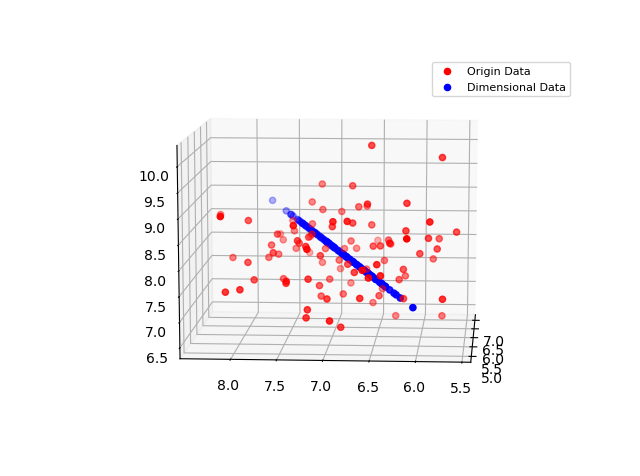
\includegraphics[width=0.7\textwidth]{3d-1d-1.png}
    }
    \subfigure[三维数据降维到一维的结果(平面侧视图)]{
        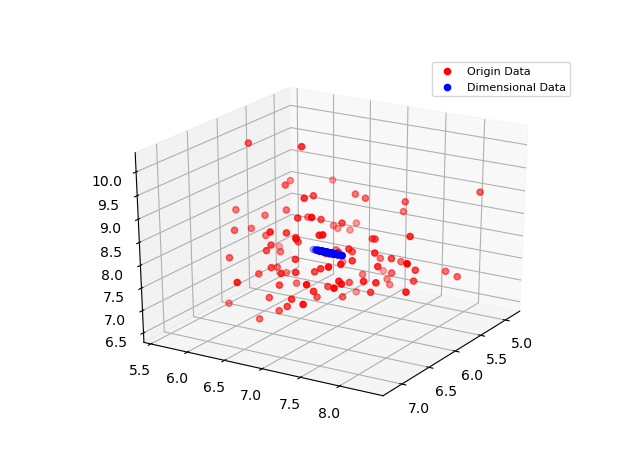
\includegraphics[width=0.7\textwidth]{3d-1d-2.png}
    }
\end{figure}
\subsection{人脸数据降维结果}
我们截取的人脸数据共有3600个维度,我们分别对其降低到1维、2维、三3维、4维和5维以及100维观察输出结果以及信噪比,原始的图像如下:
\begin{figure}[H]
    \centering
    \subfigure[原始数据]{
        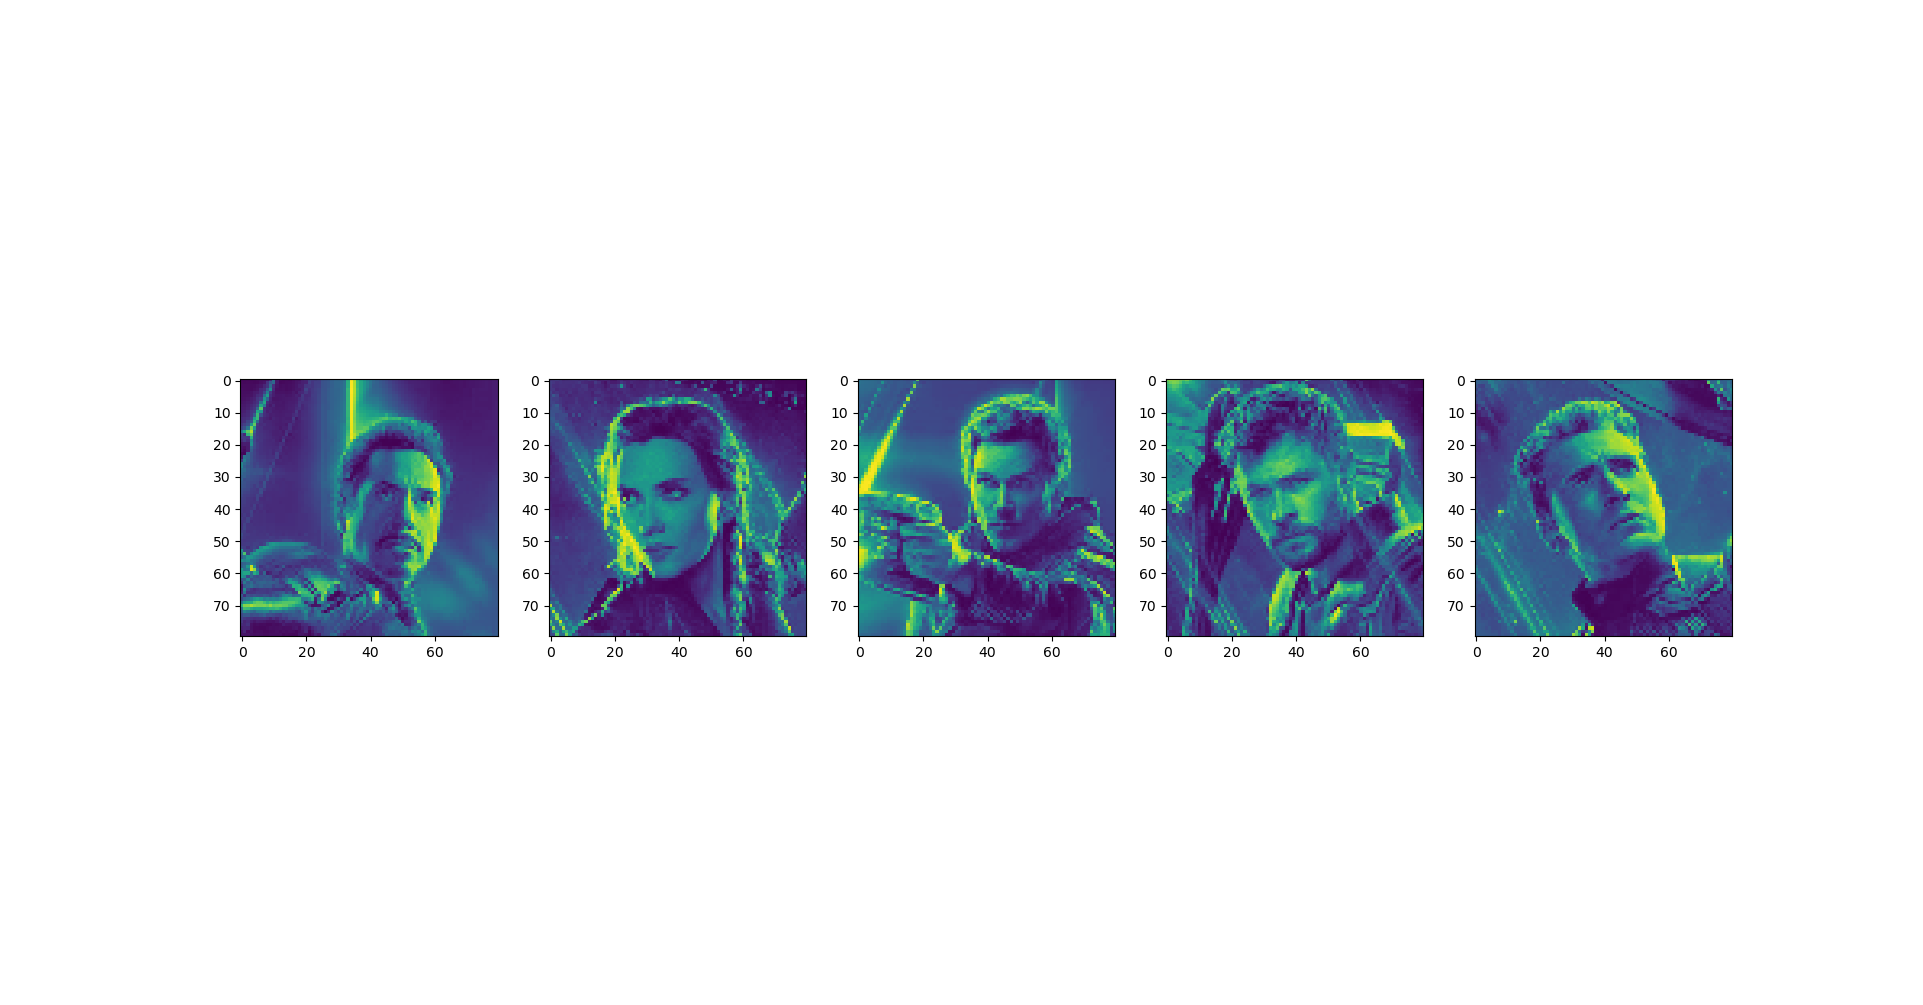
\includegraphics[width=0.8\textwidth]{origin_face_img.png}
    }
\end{figure}
\begin{figure}[H]
    \centering
    \subfigure[降低到1个维度的结果]{
        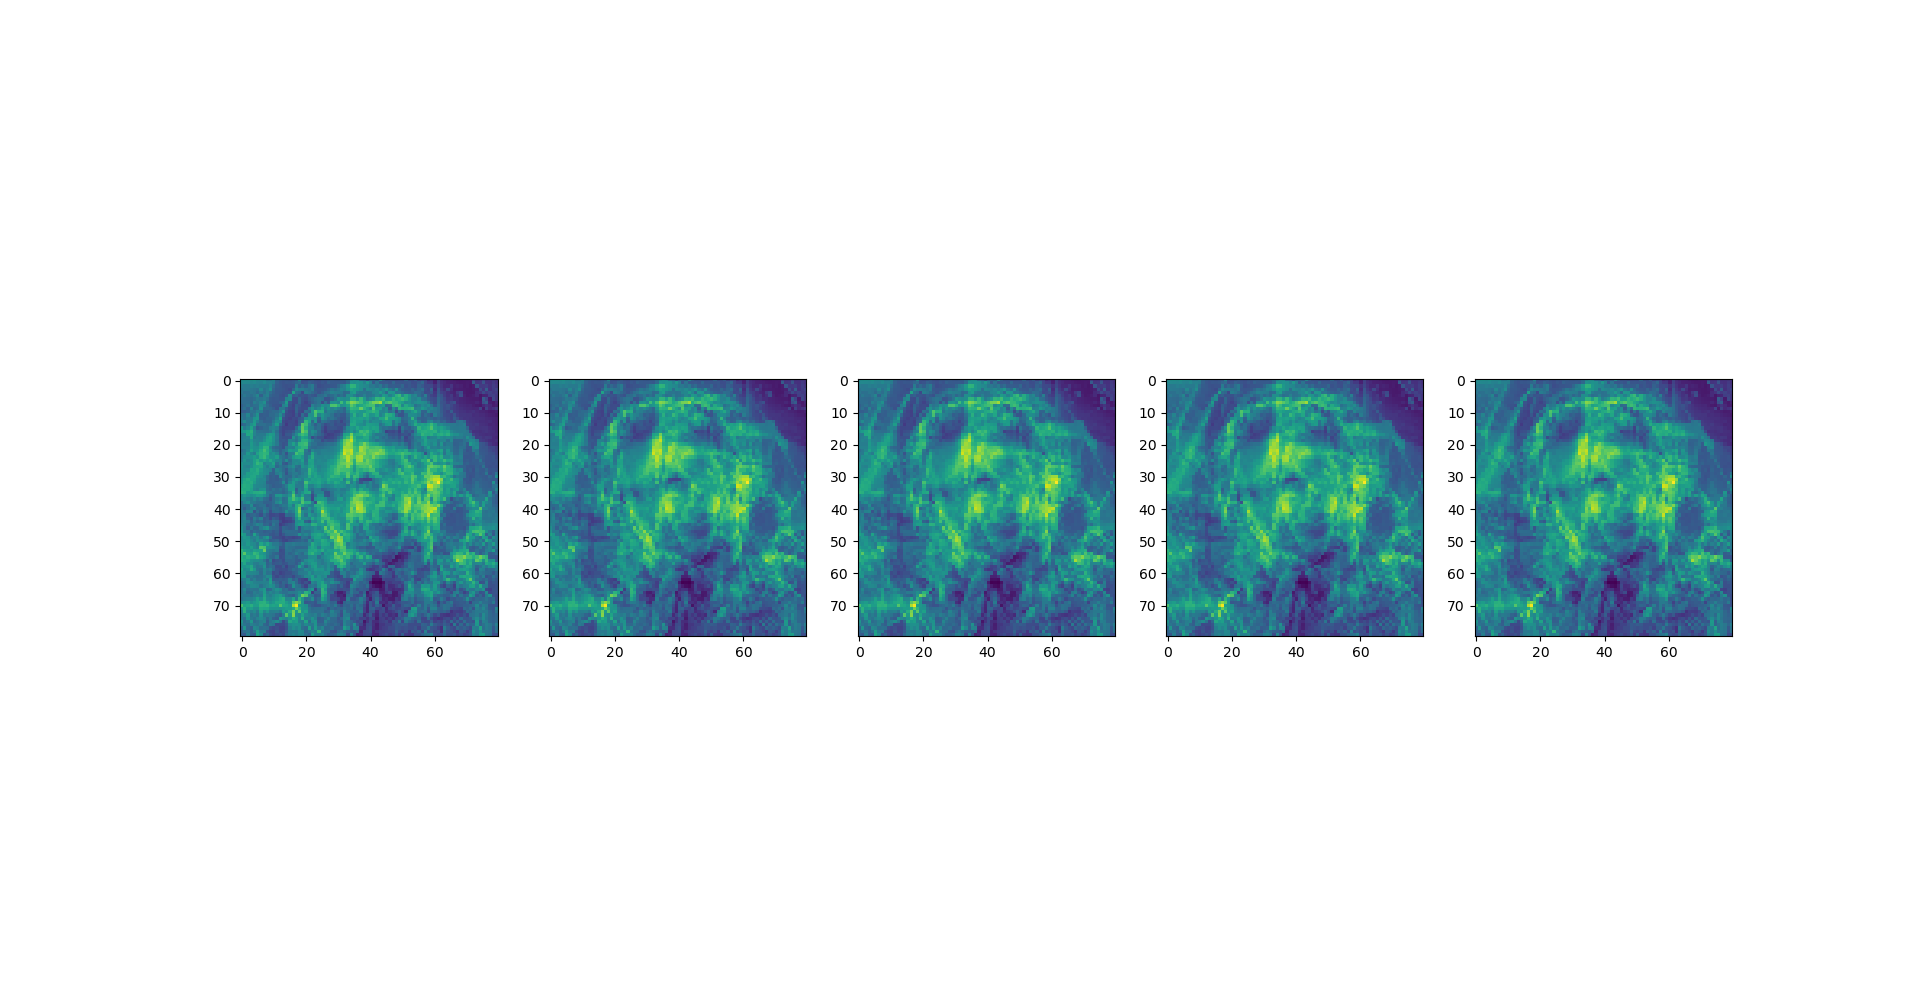
\includegraphics[width=0.8\textwidth]{to1.png}
    }
\end{figure}
由上图可以看出,降低到一个维度后的图像已经基本丧失了所有人脸特征,信噪比为14.92,难以辨认出人脸归属。
\begin{figure}[H]
    \centering
    \subfigure[降低到2个维度的结果]{
        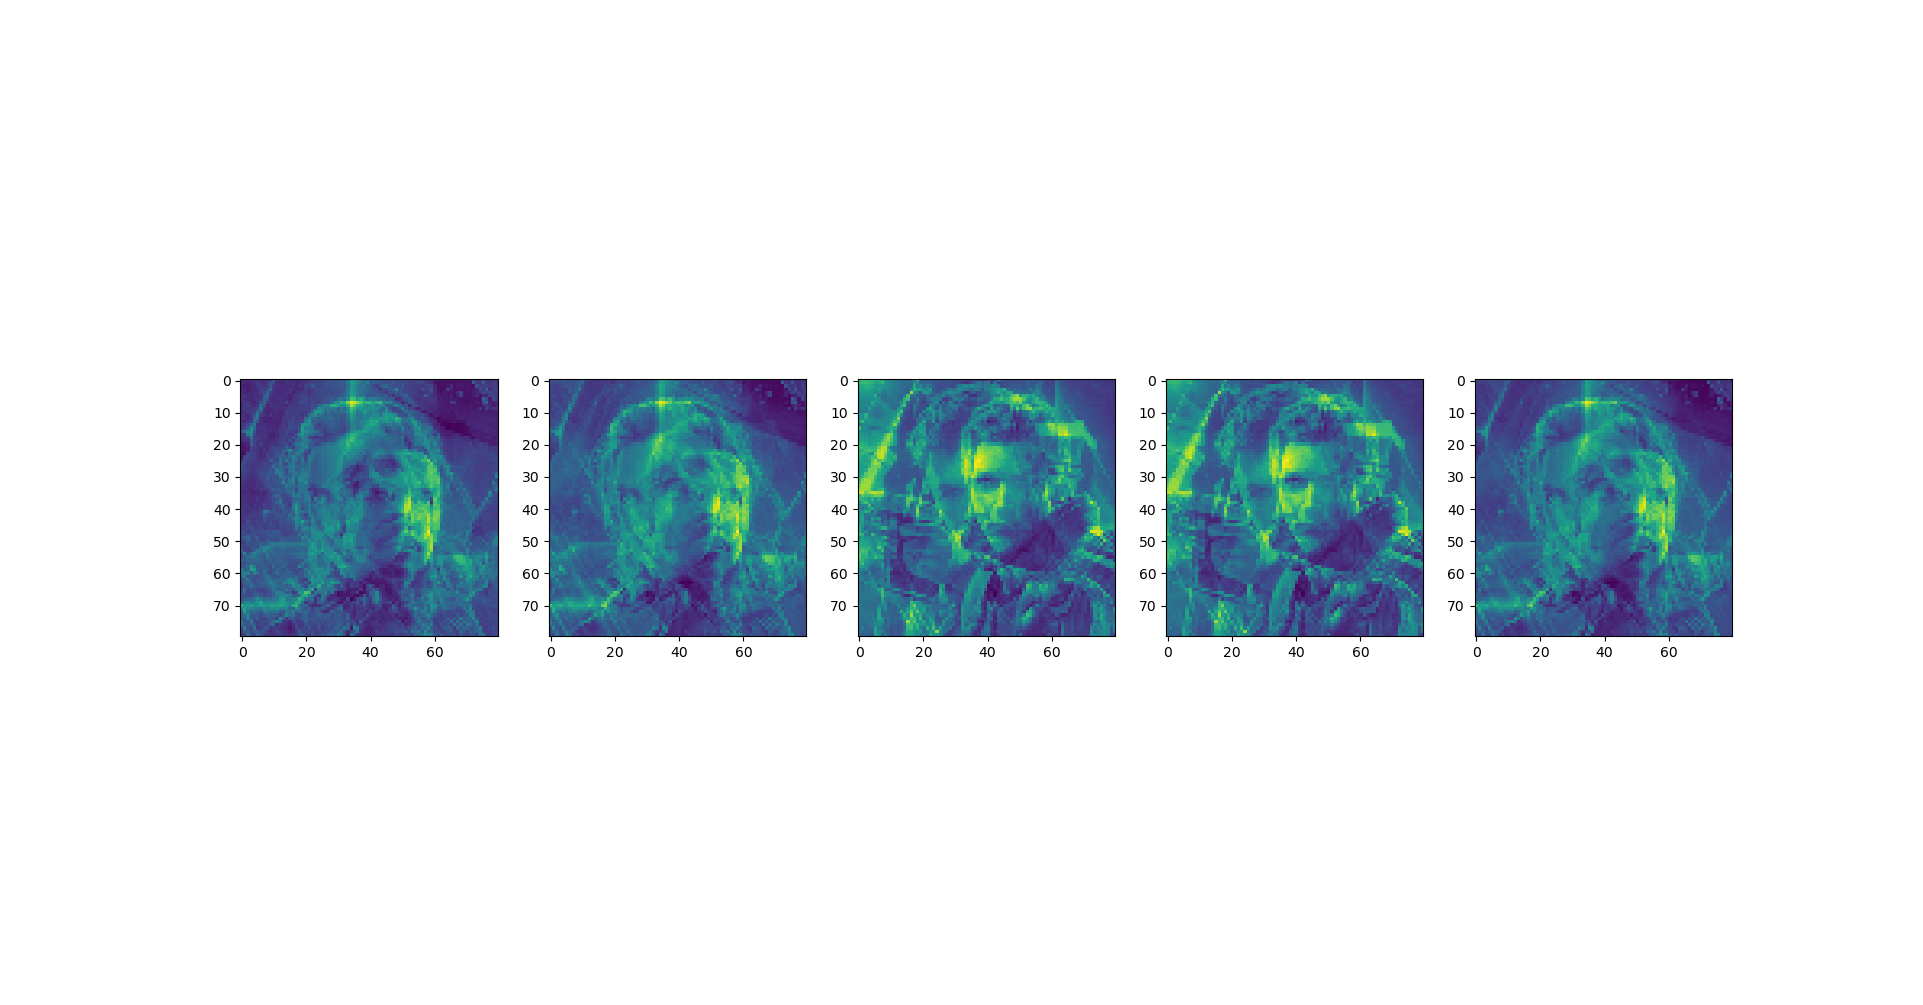
\includegraphics[width=0.8\textwidth]{to2.png}
    }
\end{figure}
降低到2个维度的数据与原数据相比也有着较大的差别,但相比于维度为1的的数据而言可以在一些地方辨认出人脸特征,信噪比为16.51。
\begin{figure}[H]
    \centering
    \subfigure[降低到3个维度的结果]{
        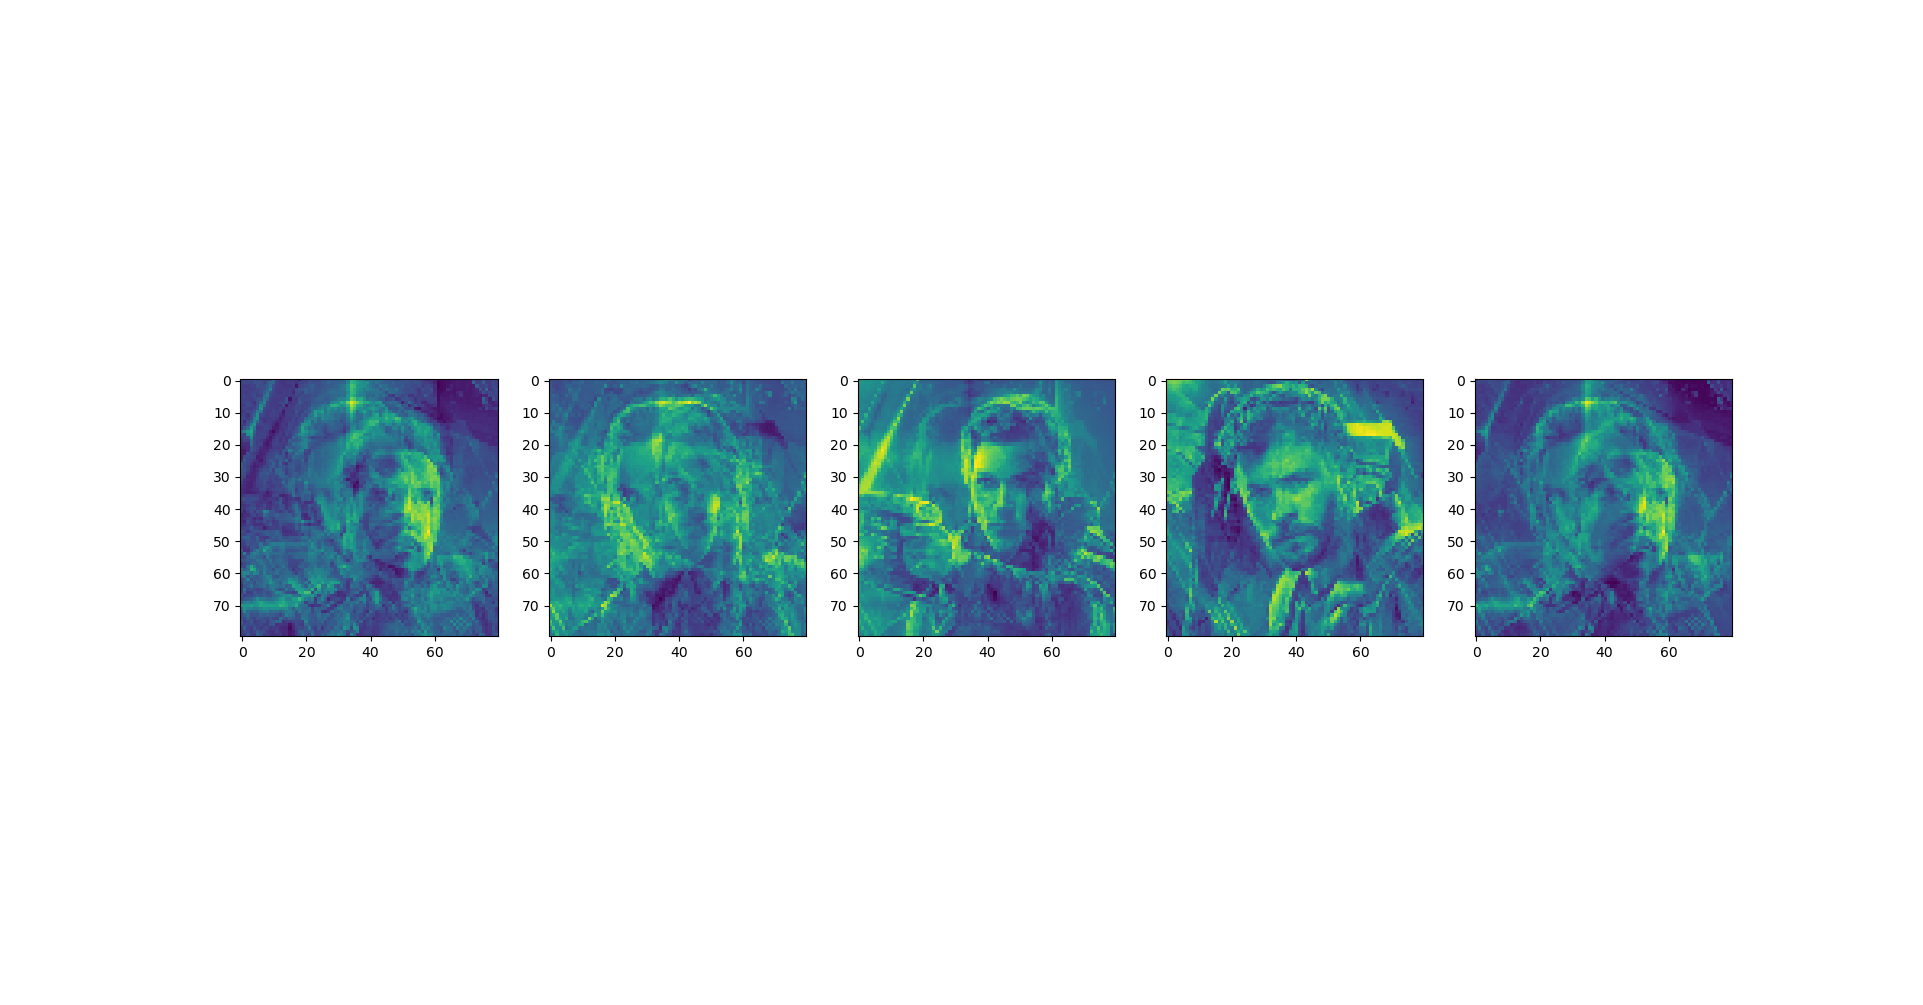
\includegraphics[width=0.8\textwidth]{to3.png}
    }
\end{figure}
降低到3个维度后,人脸特征也在一步步提升,但依旧较为模糊,信噪比为18.59。\par
\begin{figure}[H]
    \centering
    \subfigure[降低到4个维度的结果]{
        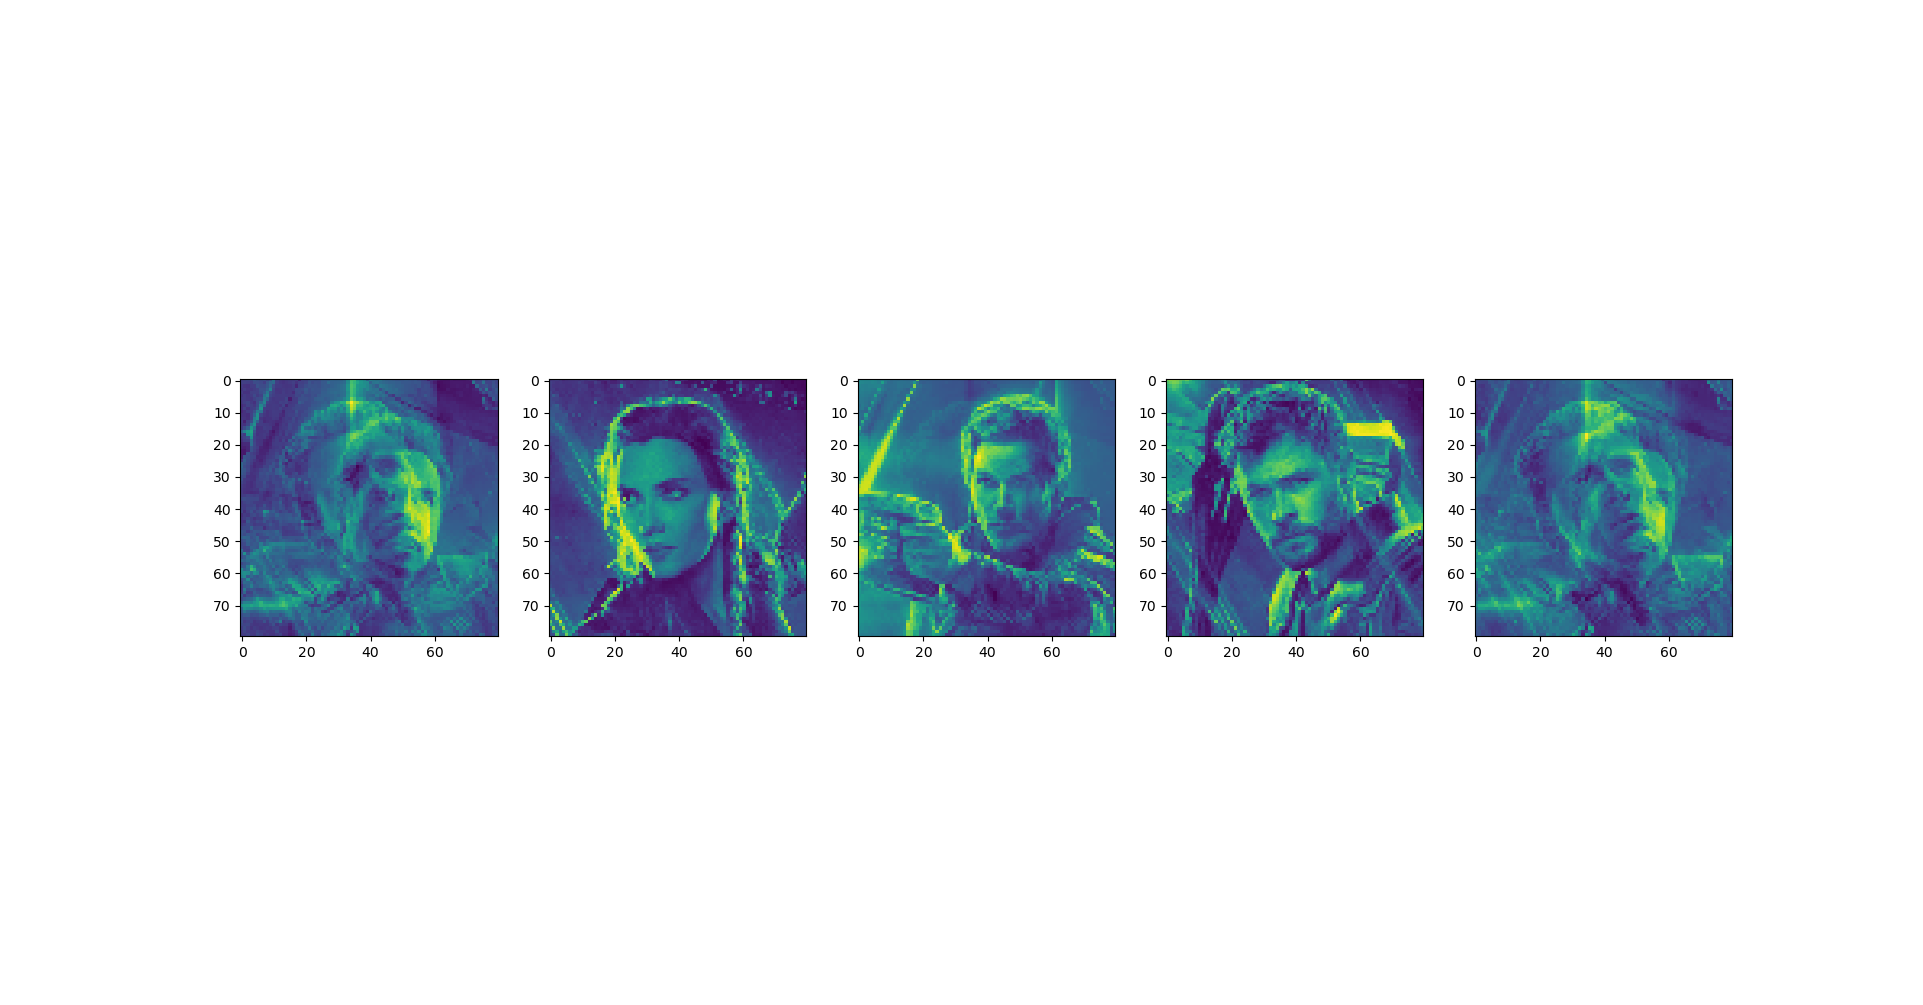
\includegraphics[width=0.8\textwidth]{to4.png}
    }
\end{figure}
降低到4个维度后,我们已经能较为完全地辨认出人脸特征,此时信噪比为22.60。\par
\begin{figure}[H]
    \centering
    \subfigure[降低到5个维度的结果]{
        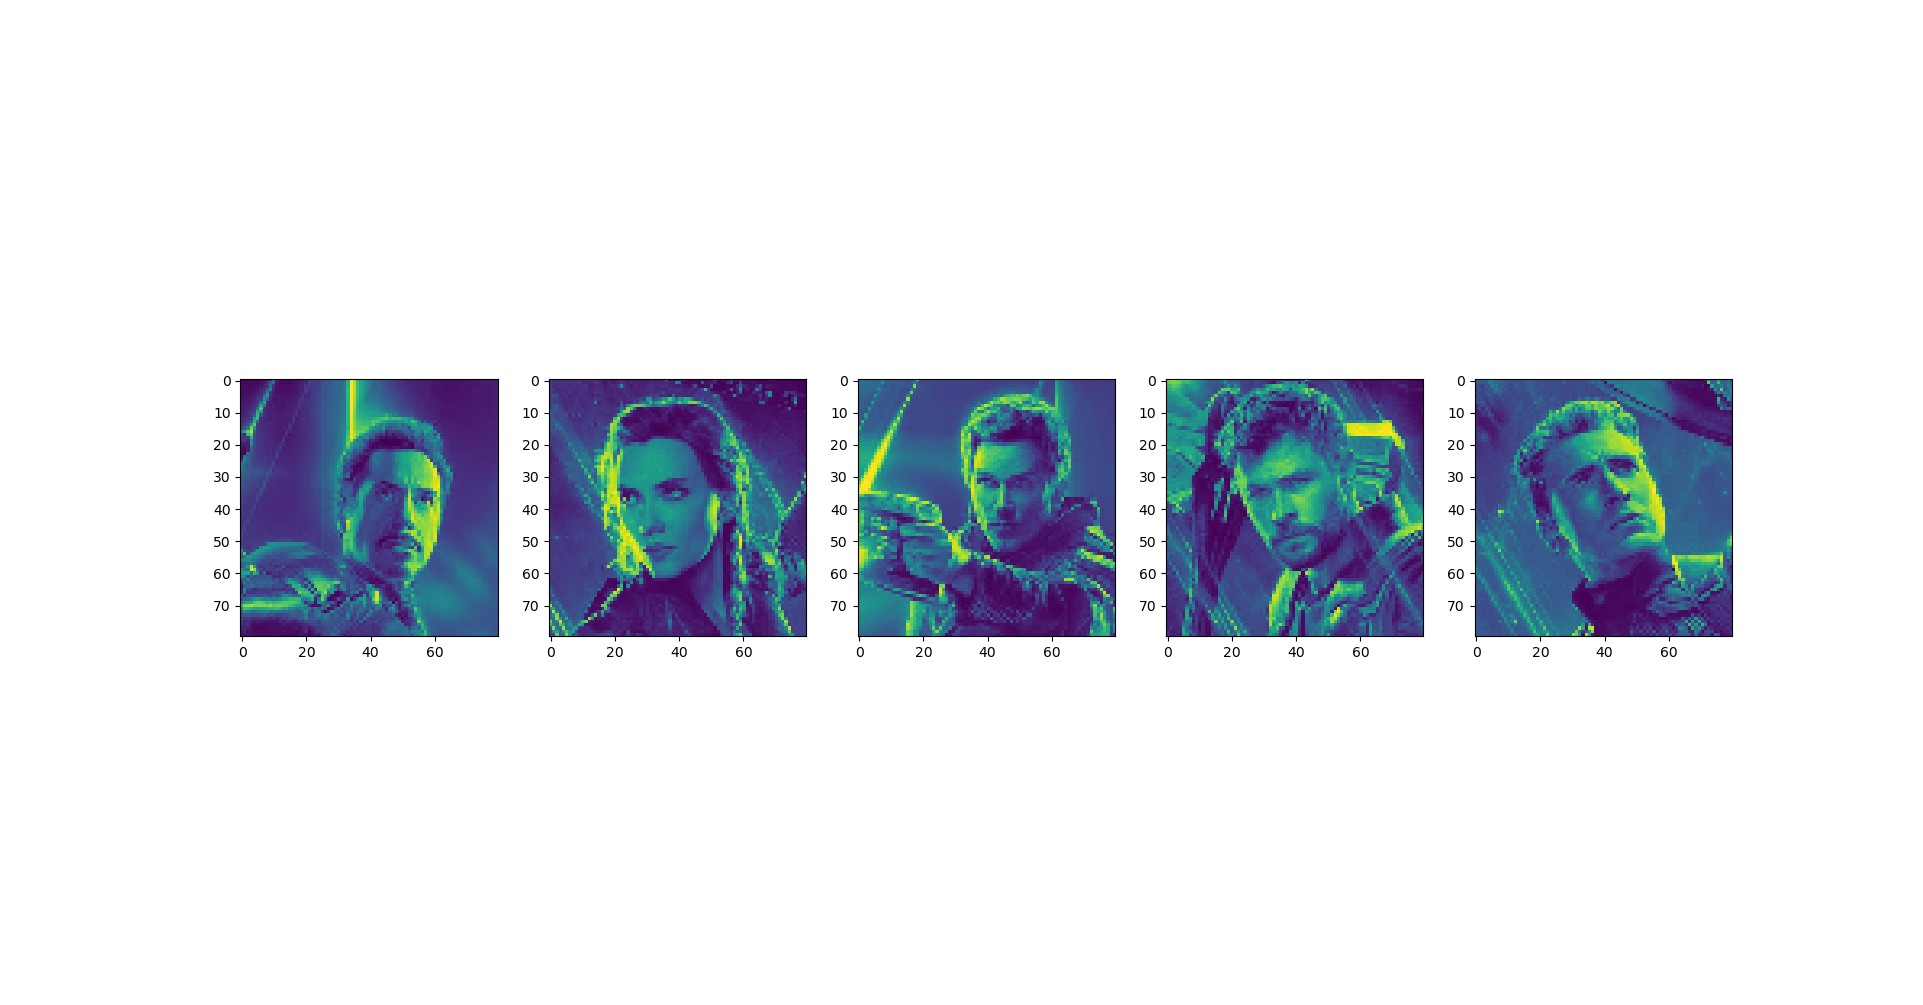
\includegraphics[width=0.8\textwidth]{to5.png}
    }
\end{figure}
降低5个维度后,我们惊奇地发现,人脸数据与原数据相比已经恢复地十分全面,没有什么太大的差别,信噪比为154.17。这大概使我们确认,5个维度就能较为完全地保存数据特征,作为比较,我们输出降低到100维的结果进行比对:\par
\begin{figure}[H]
    \centering
    \subfigure[降低到100个维度的结果]{
        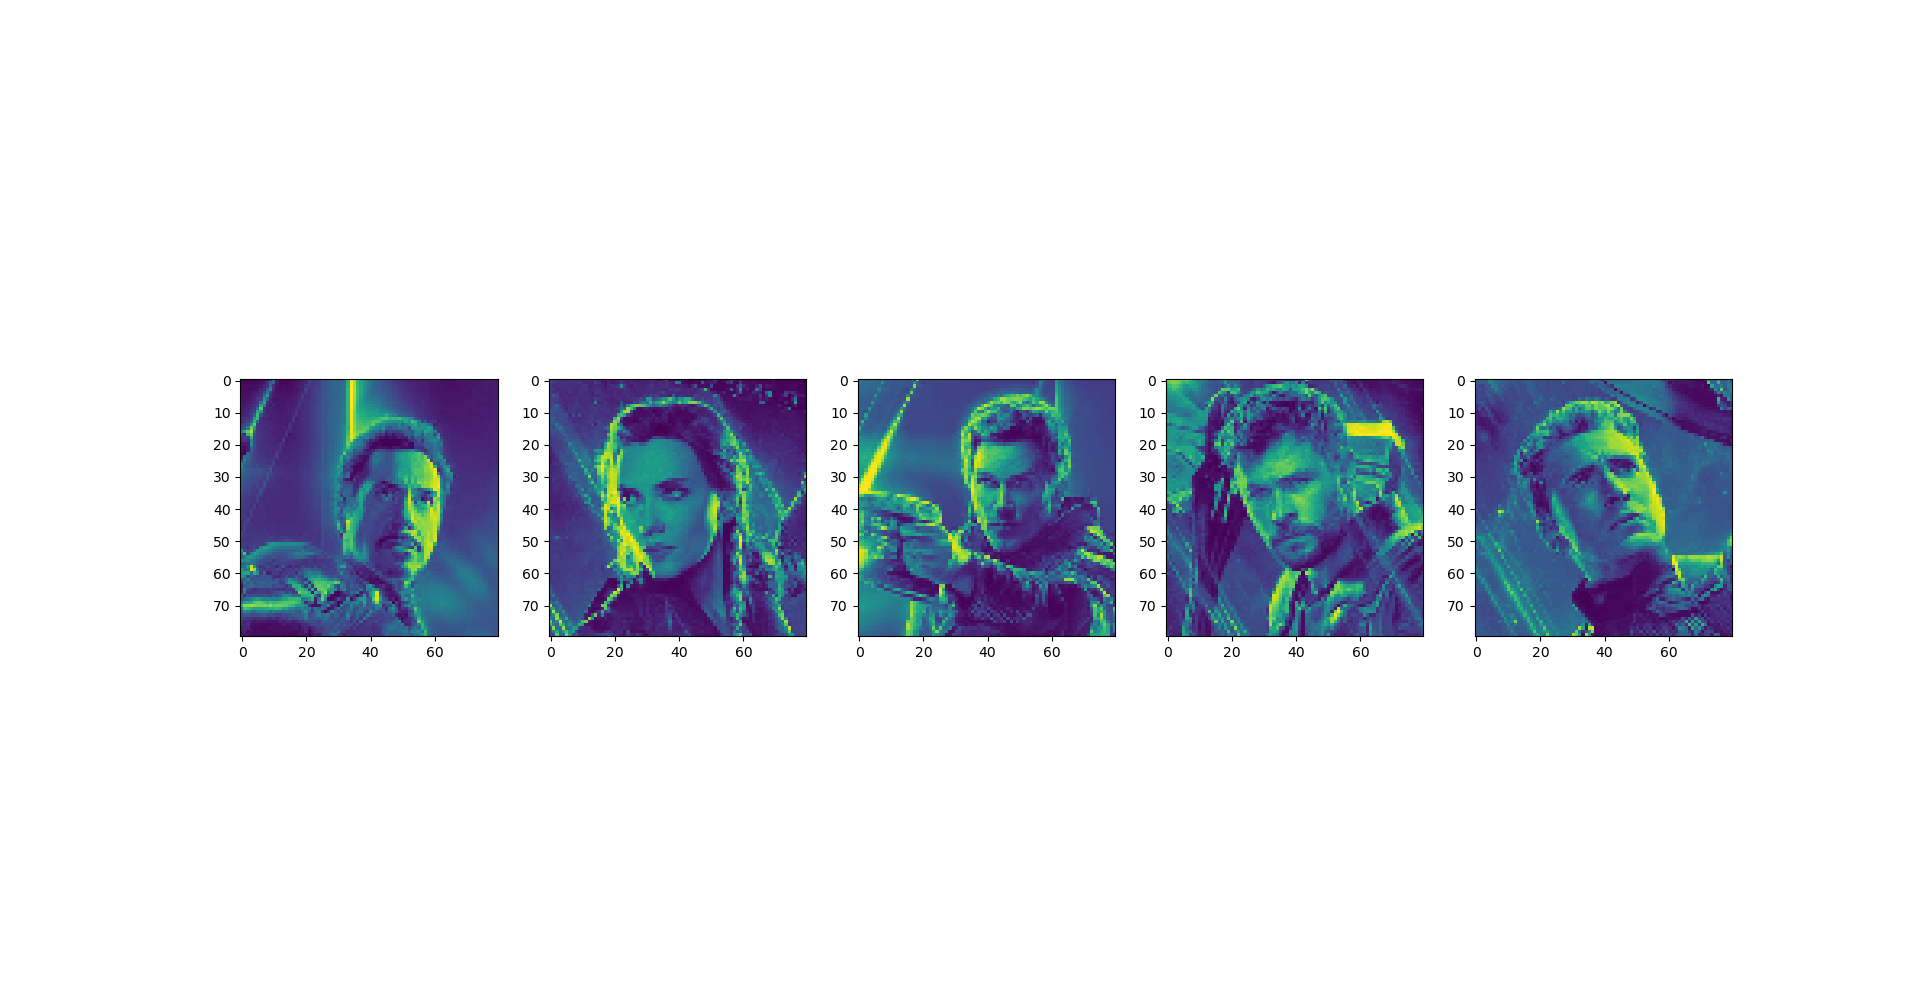
\includegraphics[width=0.8\textwidth]{to100.png}
    }
\end{figure}
此时的信噪比为154.17,与降低到5维相比差距并不大,这也印证了我们之前的推论。\par
由以上几个结果对比而言,我们可以发现降低的维度越多,信噪比越低,但当维度到达一个值的时候,就足以刻画大多的数据特征,更多的提供维度也不能明显提高信噪比了。\par
\section{结论}
在很多时候高维的数据对于数据的分析会带来很多的不便,复杂的模型与漫长的分析时间极大降低了效率。由此提出的主成分分析方法,能够在所有维度中选出能够最完全表示原来数据集的维度,通过低维度的表达尽可能的模拟表示原来的信息。通过最近重构性和最大可分性选出主成分表示数,尽可能地减少数据丢失。\par
显然,低维空间和高维空间必有不同,因为对应于最小的n-d个特征值的特征向量被舍弃了,这是降维所导致的必然结果,但舍弃这部分信息能够在其他方面带来更多的优势。一方面,舍弃这部分信息能使样本的采样密度增大,这是降维的重要动机!另一方面,当数据收到噪声影响时,最小的特征值对应的特征向量往往与噪声有关,舍弃这部分向量在一定程度上起到了降噪的作用。
\end{document}